\section{方法描述}

本节首先介绍句子和图片的输入方式,来解释如何做到明确的视觉信息作用方法。然后介绍本章设计的文本重构模型是如何工作的。最后介绍如何利用文本重构模型帮助提升翻译模型的翻译质量。

\subsection{实体替换的多模态序列}
\label{sec:3_entity_replacement}

\begin{figure}[!htbp]
    \centering
    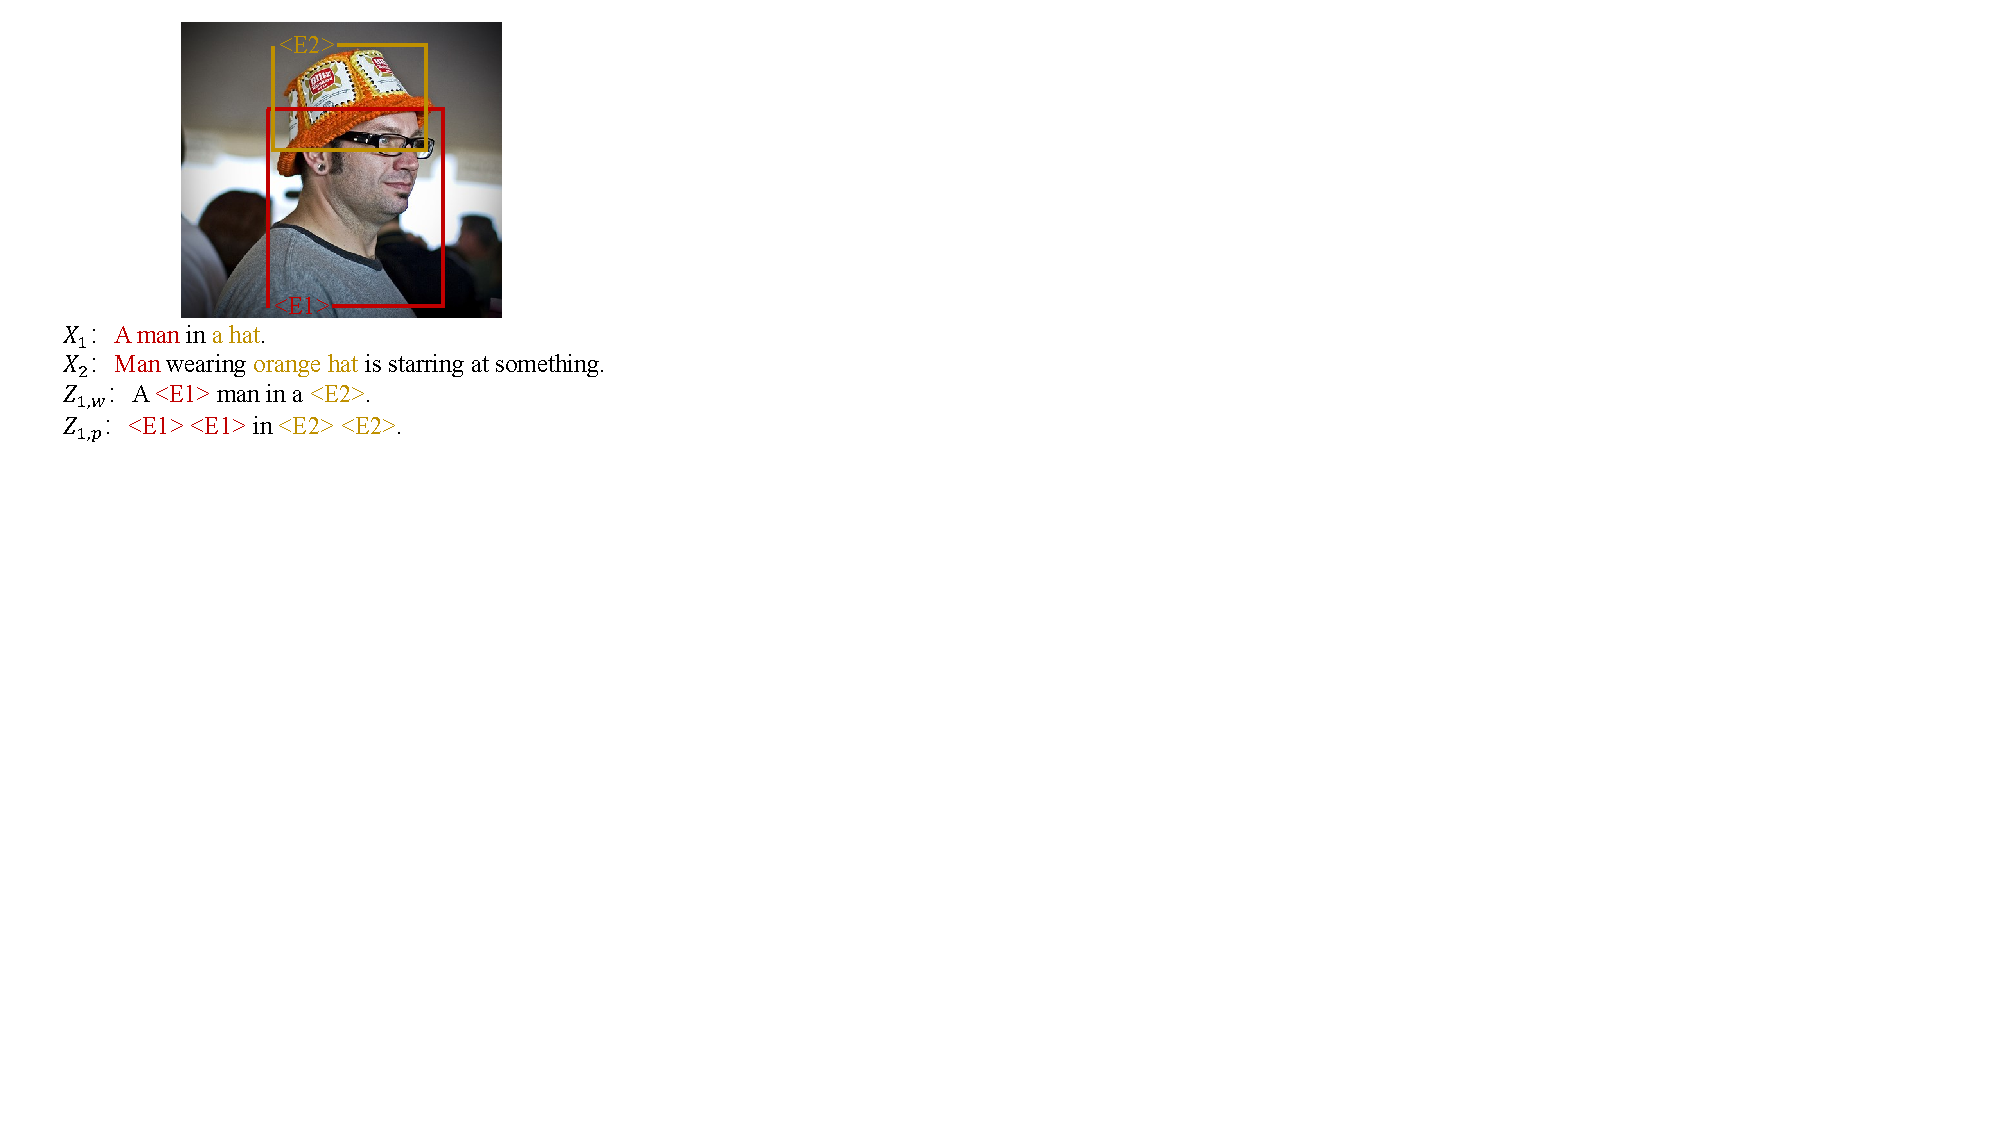
\includegraphics{Img/fig_3_example.pdf}
    \bicaption{词实体与短语实体替换示例}{An example of the word entity and the phrase entity}
    \label{fig:3_example}
\end{figure}
本章所提的句子-图片融合方法将作用于句子中的实体,为此我们以两种语义粒度定义文本实体:

(1){\sffamily 短语实体:}一个短语实体是一个视觉可描述短语,其能够完整的描述一个视觉目标图片。例如,图\ref{fig:3_example}中红框中的人“<E1>”在句子$X_1$中被描述为“A man”。其中,“man”是视觉目标,“A”为“man”的数量修饰词,两个词对于所描述的视觉目标均是有明确意义的。

(2){\sffamily 词实体:}一个词实体是短语实体中的名词实体。对于不同的描述者,视觉目标图像可以被描述为不同的短语。如图\ref{fig:3_example}中,同样是视觉目标“<E1>”,在句子$X_2$中则被描述为“Man”,对视觉目标“<E2>”,$X_1$中描述为“a hat”,在$X_2$中则使用了修饰词“orange hat”。为了消除修饰词所带来的影响,在此方案中只考虑名词作为文本实体。

本章所提的明确的图片信息融合方法,就是将源语言句子中的文本实体直接替换为图片中与文本实体相对应的视觉目标。
由于存在两种文本实体,因此本文设置两种针对句子-图片融合方法的替换规则:短语级替换规则(phrase-level replacement rule,PRR)和词级替换规则(word-level replacement rule,WRR)。在PRR中,将短语内部的所有词逐个用该短语所对应的视觉目标图像替换。例如图\ref{fig:3_example}中,$Z_{1,p}$中的“A”和“man”均被替换为“<E0>”对应的视觉目标。WRR与上述方法相似。如图\ref{fig:3_example}中$Z_{1,w}$仅名词部分(“man”,“hat”)被替换为对应的视觉目标(“<E1>”,“<E2>”)。最后的输入为该退化的句子与视觉目标图像的混合序列。

\subsection{文本重构模型}
\label{sec:3_sentence_reconstruction}
\begin{figure}[!htbp]
    \centering
    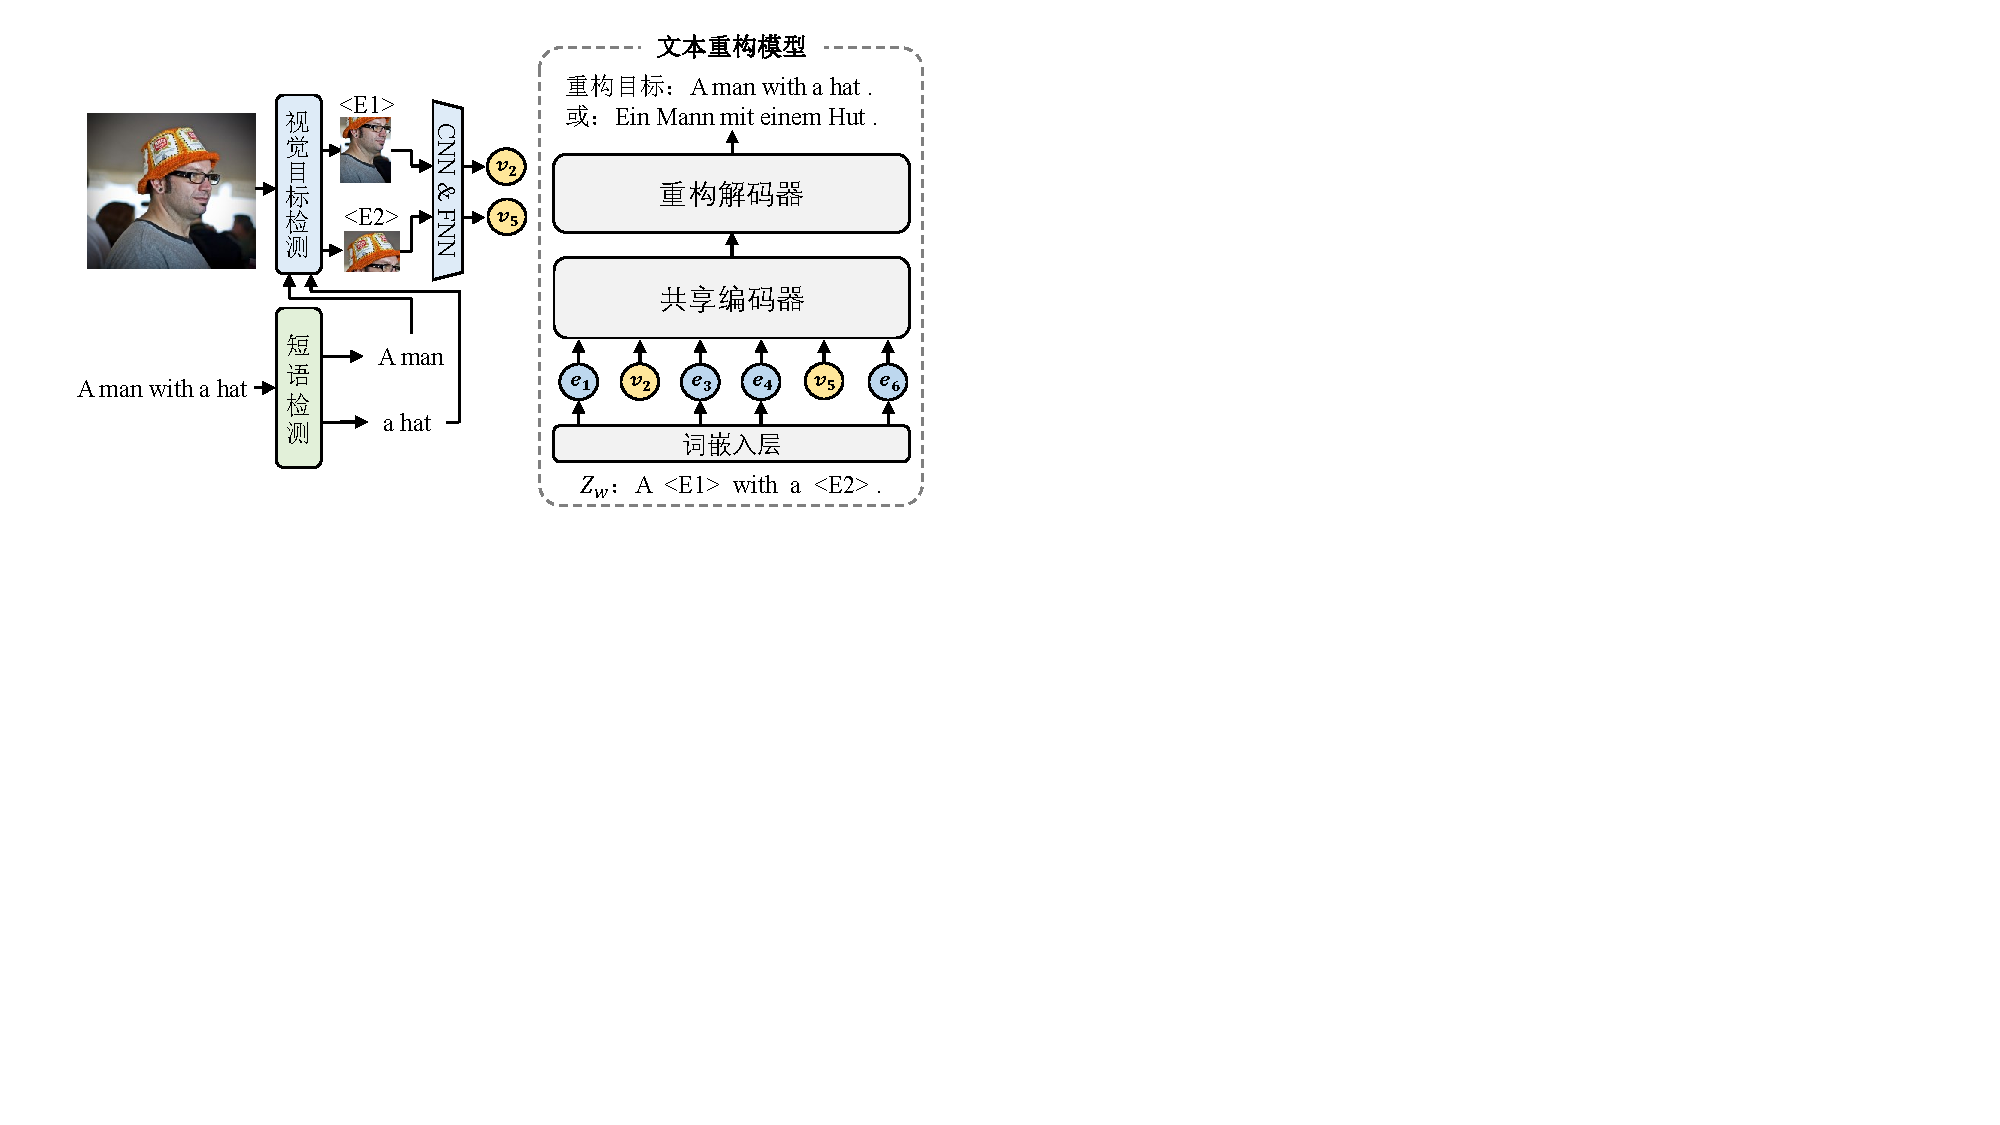
\includegraphics[scale=1.0]{Img/fig_3_reconstruction_model.pdf}
    \bicaption{融合视觉目标信息的文本重构方法}{Text reconstruction by fusing visual object information}
    \label{fig:3_reconstruction_model}
\end{figure}
为了充分利用文本模态和视觉模态的信息,本章设计了文本重构模型使显式跨模态信息融合方法有效。如图\ref{fig:3_reconstruction_model}所示,左侧为利用图\ref{fig:3_entity_extraction}中的方法提取出视觉目标后,再通过预训练的卷积神经网络提取得视觉目标的全局特征,并利用一个前馈神经网络(feedforward neural network, FNN)映射到所需要的维度。图\ref{fig:3_reconstruction_model}右侧的 “文本重构模型”是一个与“翻译模型”相似的序列到序列的生成模型。其多模态输入序列$Z_{w}$是利用WRR得到的退化文本与视觉目标图像的混合序列。该序列的向量表示为$\{\Vector{e_1,v_2,e_3,e_4,v_5,e_6}\}$。重建任务负责从$Z_{w}$重构回原始文本$X=\{x_1,x_2,…,x_N\}$。模型因此可以分别在编码阶段的视觉特征空间和在解码阶段从语言特征空间学习到实体信息。重建模型的训练方式为最小化以下对数似然方程:
\begin{equation}
    \mathcal{L}_R(\theta, \psi)=-\sum_i^N \log p(x_i|x_{<i},Z)
    \label{eq:3_reconstruction_x}
\end{equation}
其中$Z$可以是使用WRR的$Z_{w}$或是采用了PRR的$Z_{p}$,$\theta$为重构模型的编码器参数,$\psi$为重构模型的解码器参数。
考虑到重构目标语言$Y=\{y_1,y_2,\cdots,y_M\}$也是一种可行方案。此时,目标函数调整为:
\begin{equation}
    \mathcal{L}_R(\theta, \psi)=-\sum_j^M \log p(y_j|y_{<j},Z)
    \label{eq:3_reconstruction_y}
\end{equation}

\subsection{与机器翻译相结合}
\label{sec:3_multitask}
图\ref{fig:3_reconstruction_model}中所展示的重构模型与一般的神经机器翻译模型相似,都是基于编码器-解码器结构的端到端生成模型。其中翻译模型的目标函数也与公式\ref{eq:3_reconstruction_x}和公式\ref{eq:3_reconstruction_y}相近:
\begin{equation}
    \mathcal{L}_T(\theta, \phi)=-\sum_j^M \log p(y_j|y_{<j},X)
    \label{eq:3_translation}
\end{equation}
其中$\phi$为神经翻译模型的解码器参数。为了结合重构任务和翻译任务,本章按照文献\cite{37_elliott-kadar-2017-imagination}的方式将两者的目标函数结合:
\begin{equation}
    \mathcal{L}(\theta, \psi, \phi)=\omega L_T(\theta, \phi) + (1-\omega)L_R(\theta, \psi)
    \label{eq:3_combine_sr}
\end{equation}
其中$\omega$是调节多任务训练比例的超参数,即当前批数据用于更新翻译模型参数的概率。相对应的,用于更新文本重构模型参数的概率为$1-\omega$。当前的多任务学习通过共享编码器参数来达到知识迁移的目的。

\subsection{参数共享策略}
\label{sec:3_parameter_sharing}
% 
\begin{figure}[!htbp]
    \centering
    \begin{subfigure}[b]{0.5\textwidth}
      \centering
      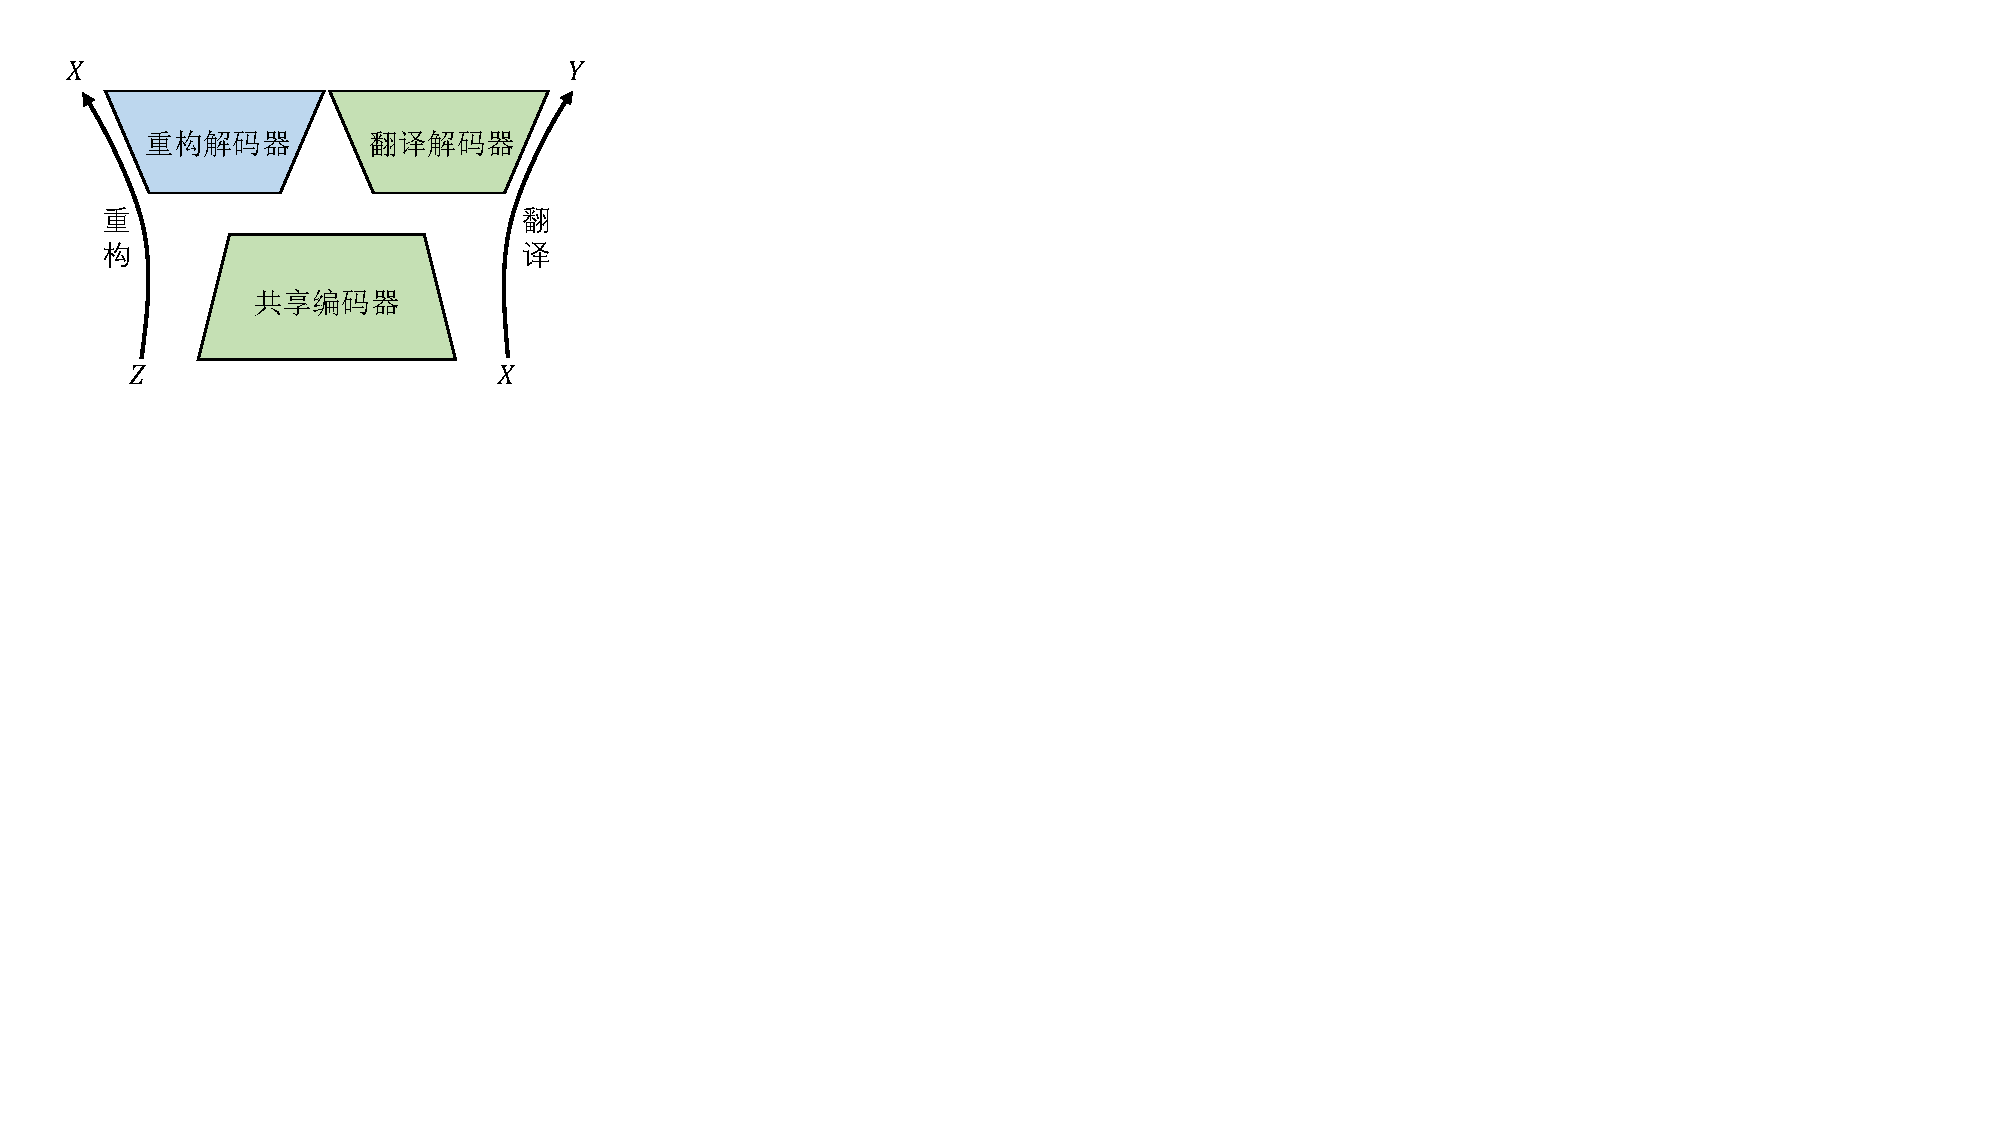
\includegraphics[scale=0.7]{Img/fig_3_sr.pdf}
      \caption{源-独享}
      \label{fig:3_sr}
    \end{subfigure}%
    ~% add desired spacing
    \begin{subfigure}[b]{0.5\textwidth}
      \centering
      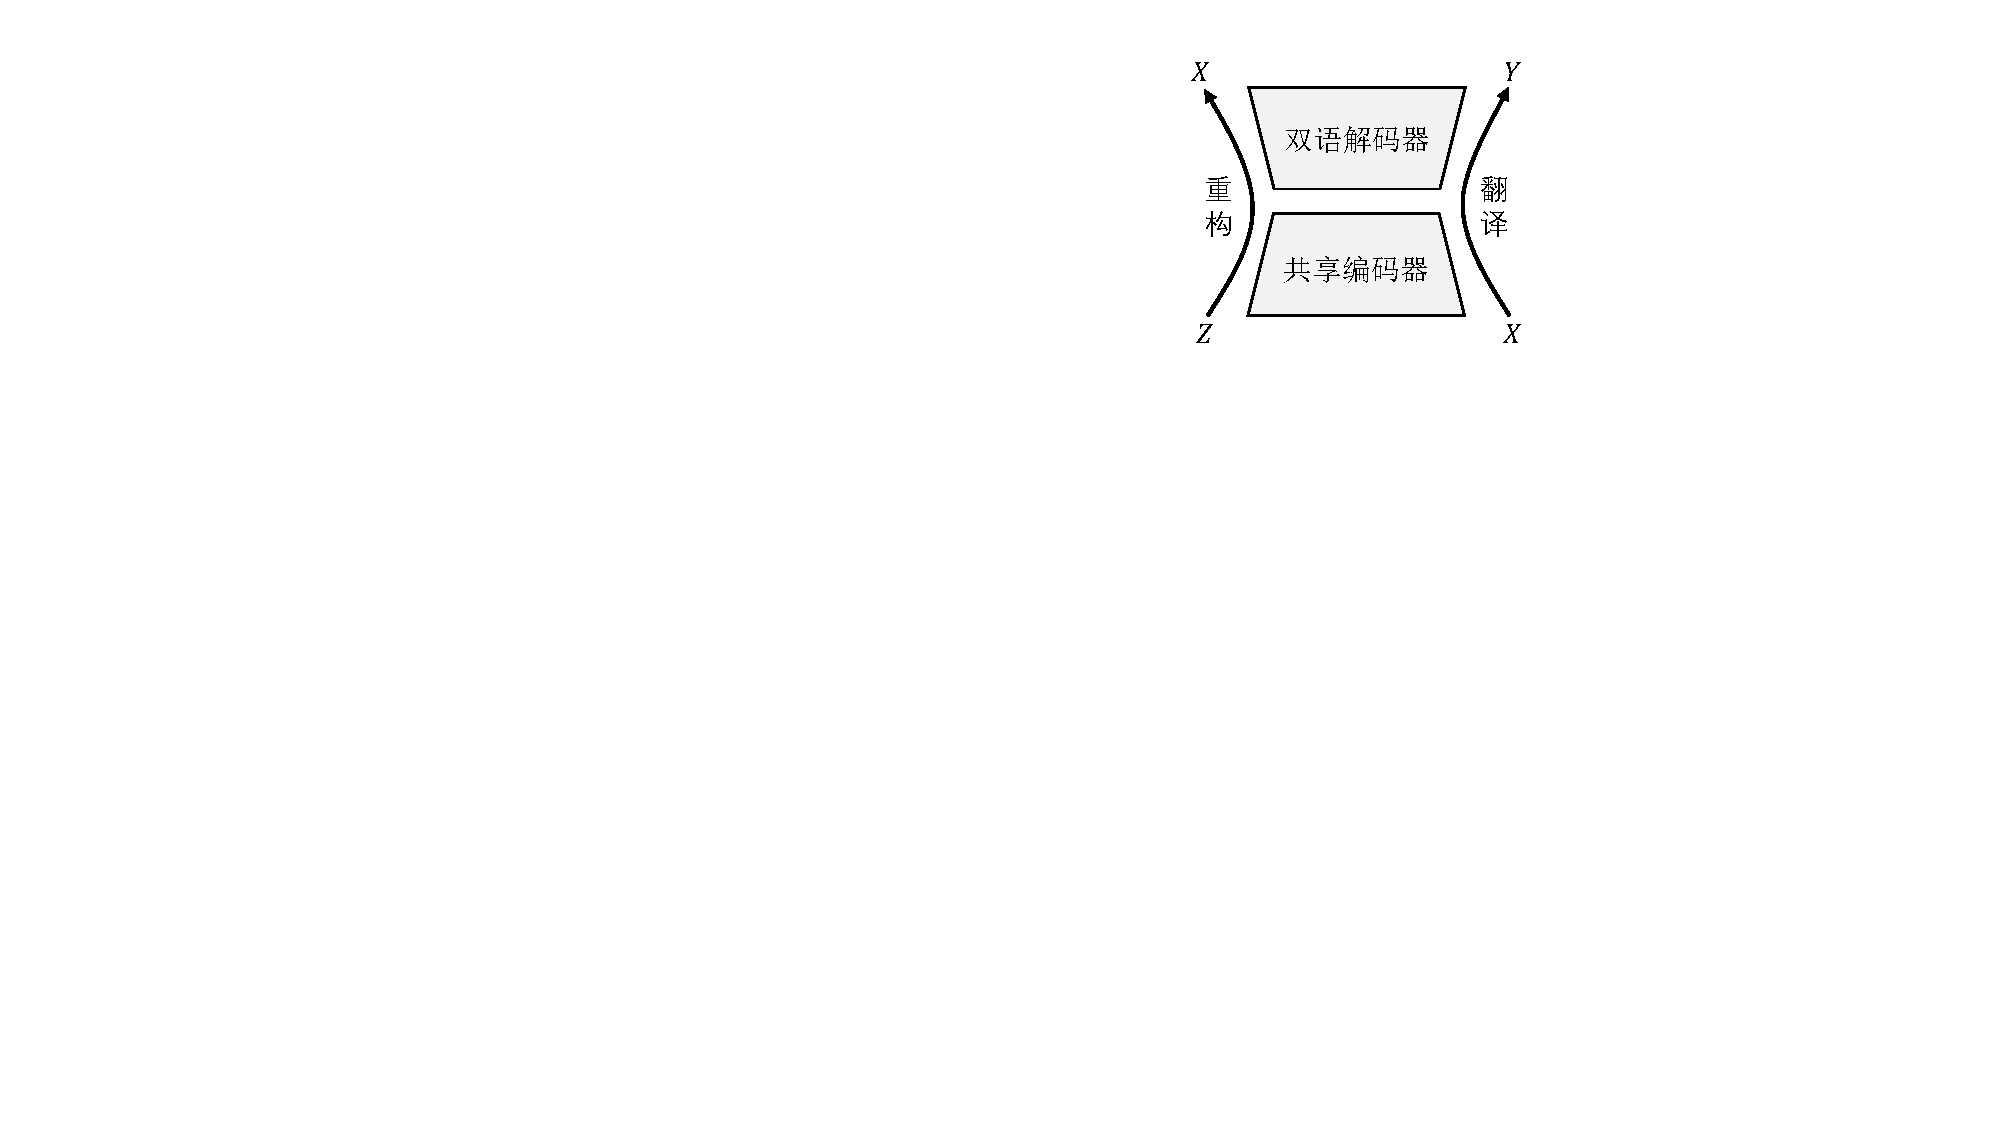
\includegraphics[scale=0.7]{Img/fig_3_ss.pdf}
      \caption{源-共享}
      \label{fig:3_ss}
    \end{subfigure}
    \\% line break
    \begin{subfigure}[b]{0.5\textwidth}
      \centering
      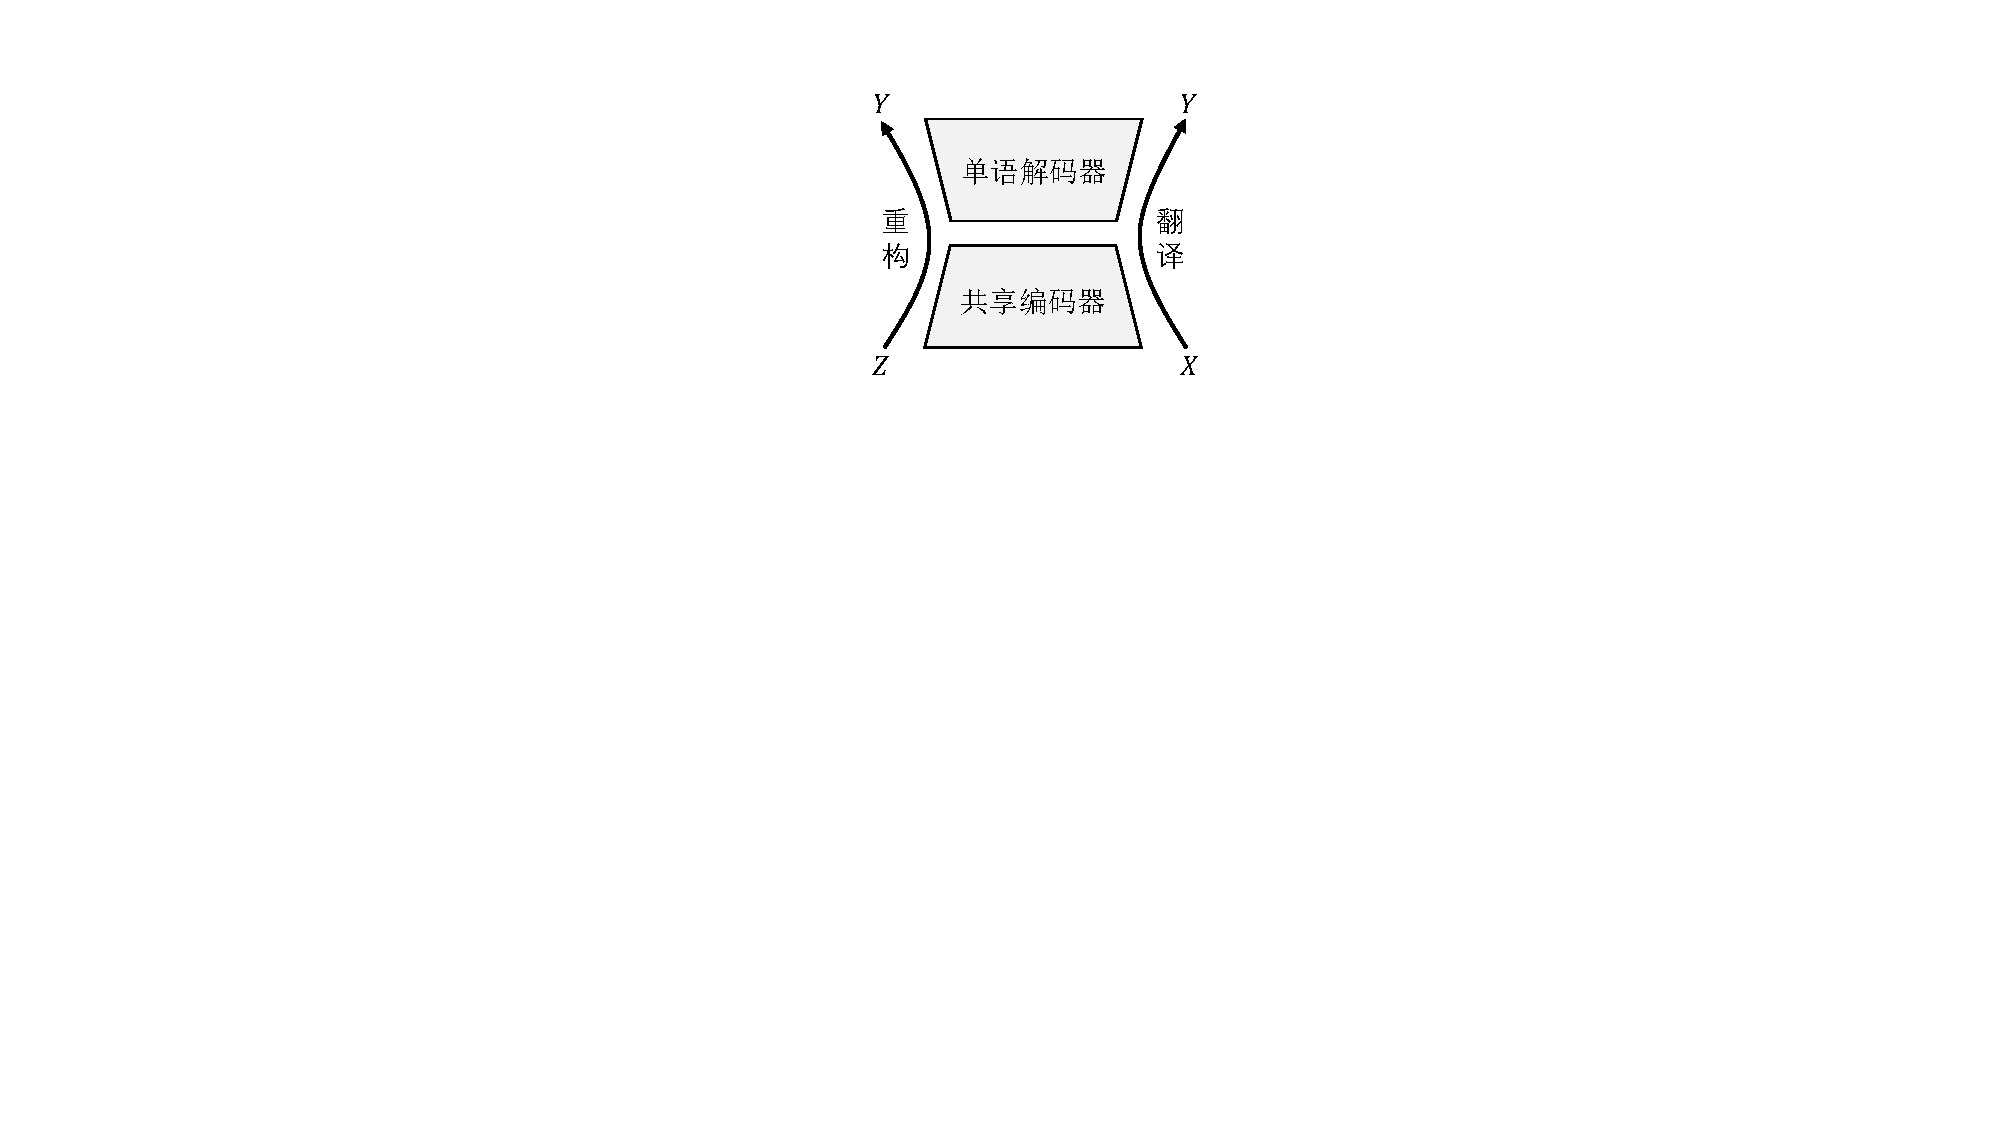
\includegraphics[scale=0.7]{Img/fig_3_t.pdf}
      \caption{目-共享}
      \label{fig:3_t}
    \end{subfigure}%
    \bicaption{重构模型与翻译模型的参数共享方案}{Parameter sharing schemes between reconstruction model and translation model}
    \label{fig:4_fidelity}
\end{figure}
正如前面章节所提到,重构模型与翻译模型在结构上有高度的相似性,因此可以利用参数共享的方法将重构模型学习到的视觉信息融合到翻译模型中,从而达到提升翻译质量的目的。因此,由编码器-解码器结构的灵活性与两种重构目标可组合得到多种参数共享方案。本文采用了以下三种参数共享方案。

(1){\sffamily 独享解码器重构源语言}
\begin{figure}[!htbp]
    \centering
    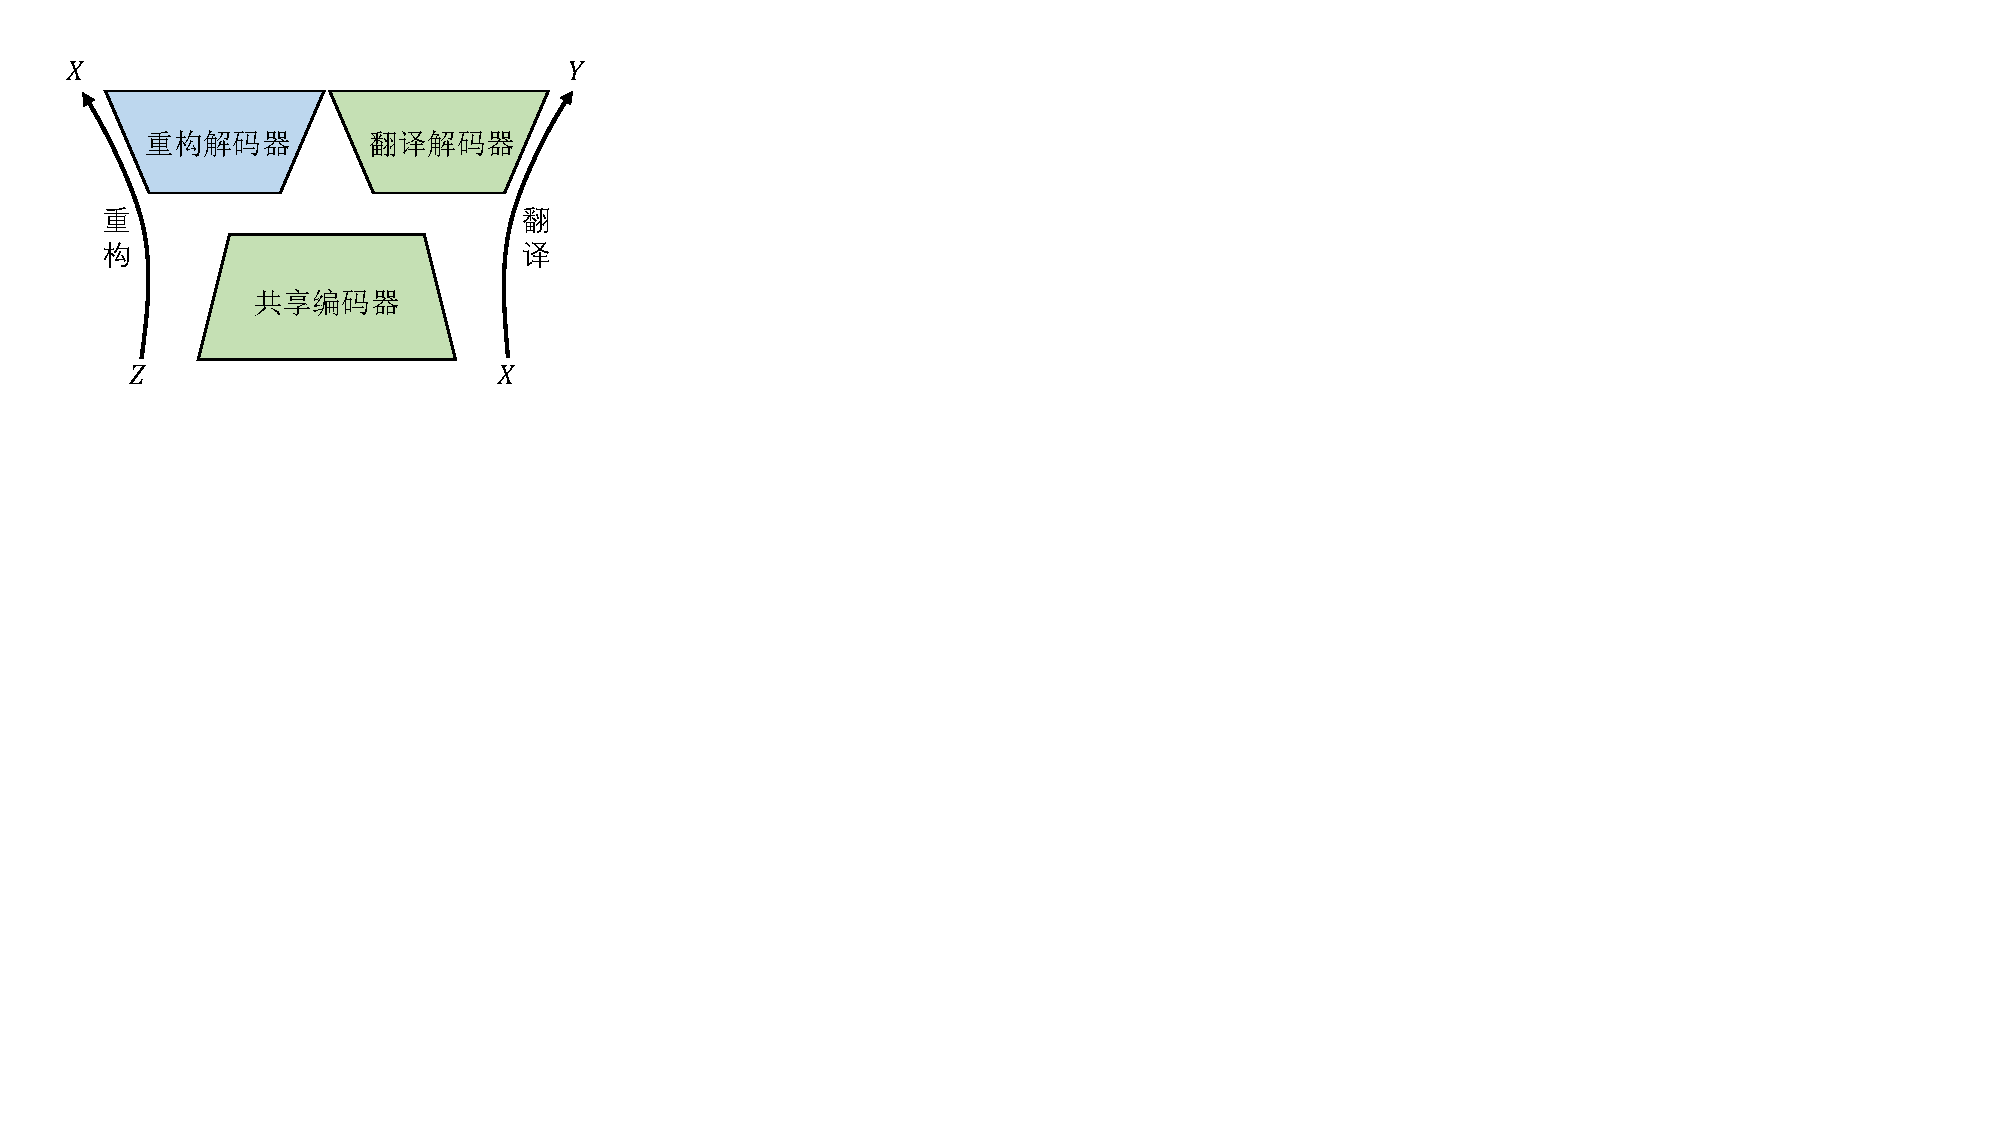
\includegraphics[scale=0.9]{Img/fig_3_sr.pdf}
    \bicaption{独享解码器重构源语言“源-独享”}{Reconstruction for source language with respective decoder}
    \label{fig:3_sr}
\end{figure}

由于视觉信息要在编码的过程中学习特征表示,因此在所有的参数共享策略中,都要包含共享编码器。解码器的参数共享则是可选的。在利用独享解码器重建源语言的策略中,为源语言和目标语言设立独立的解码器,即重构模型和翻译模型的编码器是共享的,解码器参数是独享的。联合目标函数如公式\ref{eq:3_combine_sr},在后面的实验中,本文用“源-独享”表示应用该策略。

(2){\sffamily 共享解码器重构源语言}
\begin{figure}[!htbp]
    \centering
    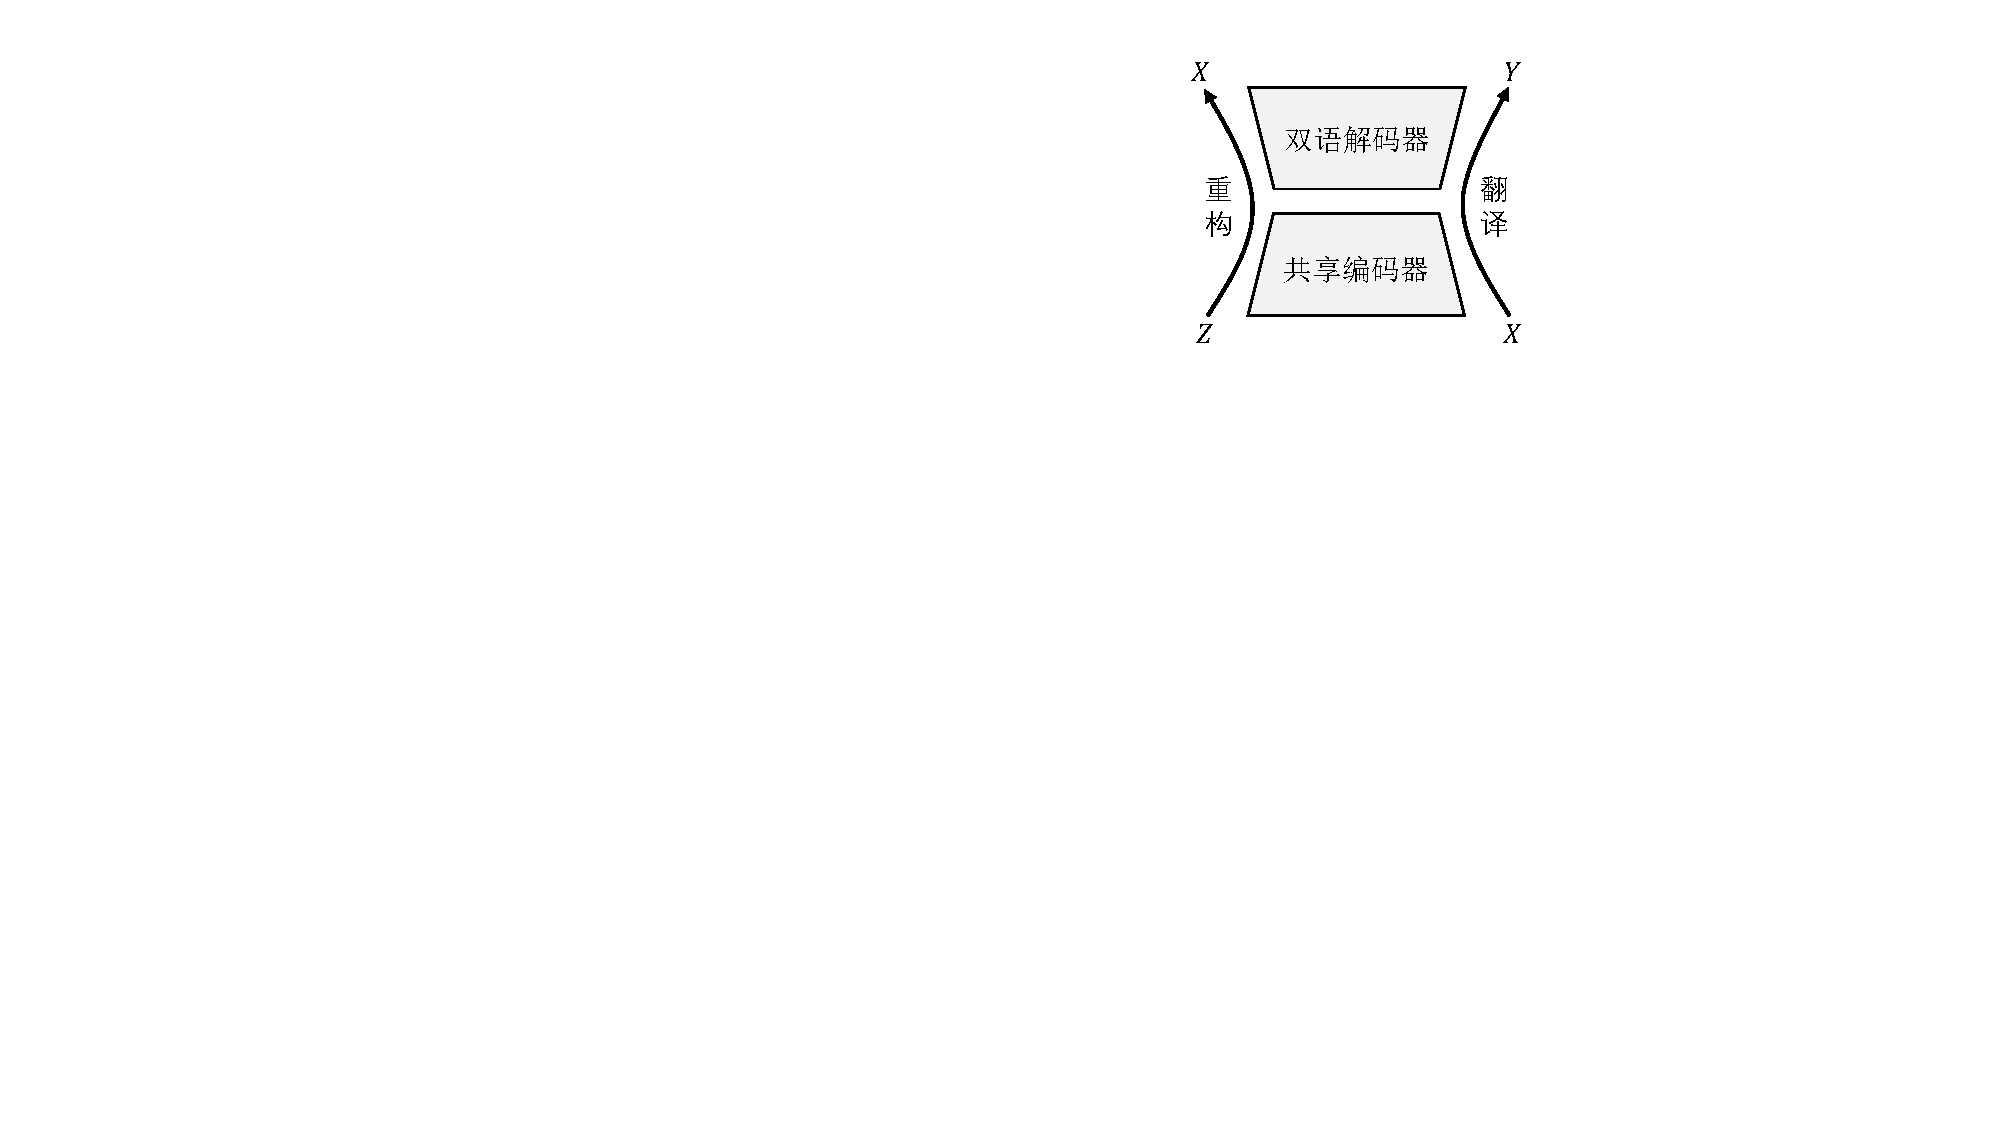
\includegraphics[scale=0.9]{Img/fig_3_ss.pdf}
    \bicaption{共享解码器重构源语言“源-共享”}{Reconstruction for source language with shared decoder}
    \label{fig:3_ss}
\end{figure}

通过融合源语言和目标语言的词表,以及在编码器和解码器之间共享词嵌入层的方式,可以实现重构模型和翻译模型的共享解码器的设置。同时,需要在解码过程目标语言句子输入时,在句首引入一个“识别词”(例如,“<en\_sos>”表示解码到英语,“<de\_sos>”表示解码到德语)用于表示当前解码器用于重构到源语言还是翻译到目标语言。在该设置中,公式\ref{eq:3_combine_sr}中有$\psi=\phi$。这表明该策略中翻译模型和重建模型是全参数共享的。因此,将联合目标函数调整为:
\begin{equation}
    \mathcal{L}(\theta, \phi)=\omega \mathcal{L}_T(\theta, \phi) + (1-\omega)\mathcal{L}_R(\theta, \phi)
    \label{eq:3_combine_ss}
\end{equation}
本文将用“源-共享”代表该参数共享策略。

(3){\sffamily 共享解码器重构目标语言}
\begin{figure}[!htbp]
    \centering
    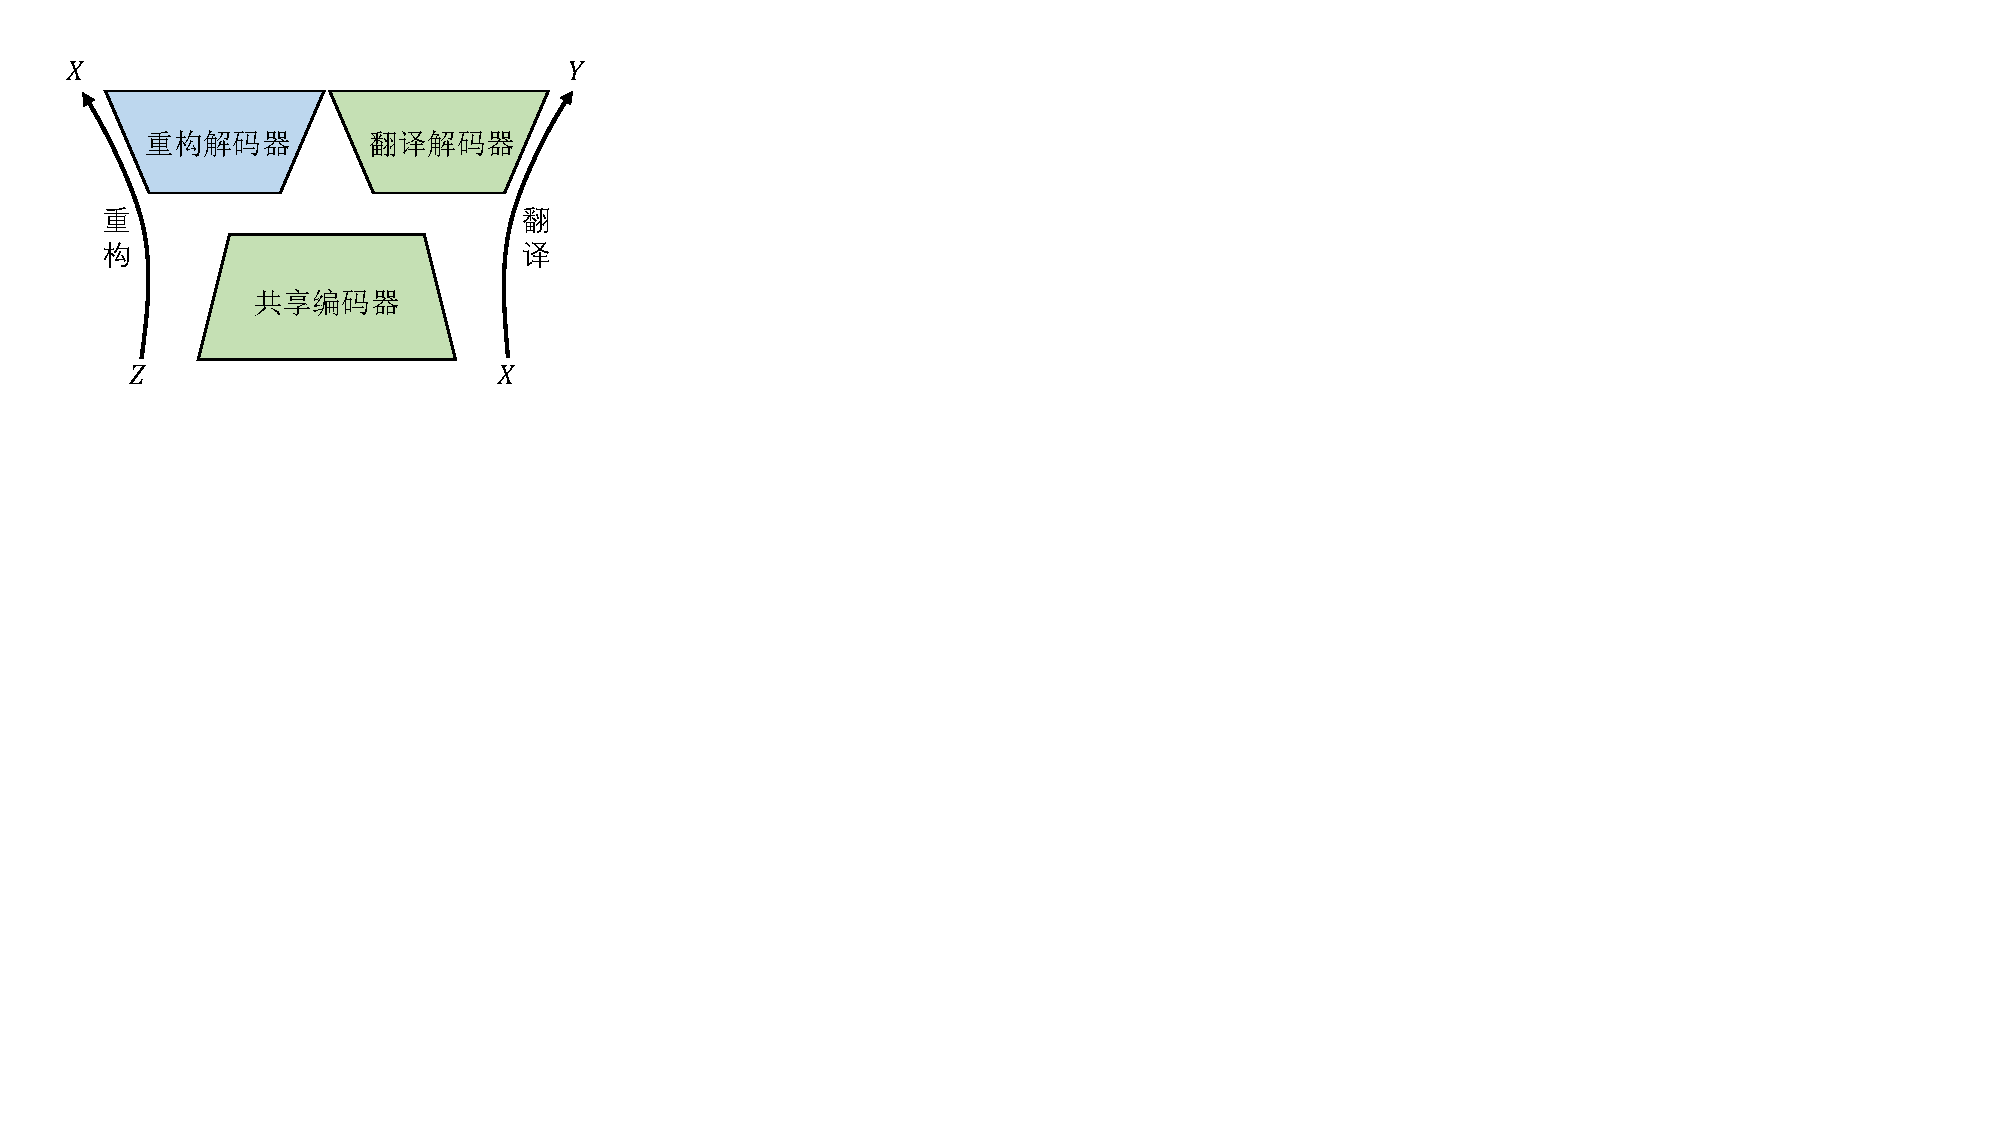
\includegraphics[scale=0.9]{Img/fig_3_sr.pdf}
    \bicaption{共享解码器重构目标语言“目-共享”}{Reconstruction for target language with shared decoder}
    \label{fig:3_t}
\end{figure}

不同于重构源语言,解码器的参数共享策略在重建目标语言的方向上则很容易实现。在该策略中,重构任务的工作方式与一般的MMT模型相似,区别在于输入的文本是退化文本。并且其联合目标函数与公式\ref{eq:3_combine_ss}相同。本文将用“目-共享”来表示该参数共享策略。